%%%%%%%%%%%%%%%%%%%% book.tex %%%%%%%%%%%%%%%%%%%%%%%%%%%%%
%
% sample root file for the chapters of your "monograph"
%
% Use this file as a template for your own input.
%
%%%%%%%%%%%%%%%% Springer-Verlag %%%%%%%%%%%%%%%%%%%%%%%%%%


\documentclass[graybox,envcountchap,sectrefs]{svmono}

% choose options for [] as required from the list
% in the Reference Guide

\usepackage{mathptmx}
\usepackage{helvet}
\usepackage{courier}
%
\usepackage{type1cm}

\usepackage{makeidx}         % allows index generation
\usepackage{graphicx}        % standard LaTeX graphics tool
                             % when including figure files
\usepackage{multicol}        % used for the two-column index
\usepackage[bottom]{footmisc}% places footnotes at page bottom
\usepackage[numbers]{natbib}


% support Chinese
\usepackage{CTex}

% see the list of further useful packages
% in the Reference Guide

\makeindex             % used for the subject index
                       % please use the style svind.ist with
                       % your makeindex program

%%%%%%%%%%%%%%%%%%%%%%%%%%%%%%%%%%%%%%%%%%%%%%%%%%%%%%%%%%%%%%%%%%%%%

\begin{document}

\author{CSLT}
\title{Kaldi 0}
\subtitle{��������ʶ��ϵͳ����뿪��}
\maketitle


\frontmatter%%%%%%%%%%%%%%%%%%%%%%%%%%%%%%%%%%%%%%%%%%%%%%%%%%%%%%

%\include{dedic}
%\include{foreword}
%\include{preface}
%\include{acknow}

\tableofcontents

%\include{acronym}


\mainmatter%%%%%%%%%%%%%%%%%%%%%%%%%%%%%%%%%%%%%%%%%%%%%%%%%%%%%%%
\include{part}
\include{chapter1}
\include{chapter2}
\include{chapter3}
%%%%%%%%%%%%%%%%%%%%% chapter.tex %%%%%%%%%%%%%%%%%%%%%%%%%%%%%%%%%
%
% sample chapter
%
% Use this file as a template for your own input.
%
%%%%%%%%%%%%%%%%%%%%%%%% Springer-Verlag %%%%%%%%%%%%%%%%%%%%%%%%%%
%\motto{Use the template \emph{chapter.tex} to style the various elements of your chapter content.}
\chapter{ǰ�˴���}
\label{intro} % Always give a unique label
% use \chaptermark{}
% to alter or adjust the chapter heading in the running head
\abstract{����ʶ��ϵͳ��Ϊǰ�˴����ͺ�˴����������֣�ǰ�˴�����Ҫ������������ȡ���������Ż������ȡ�������ȡ���Խ���ȡ�����õ���Ϣ������޹ص���Ϣ���米���������ŵ�������ȥ�����������Ż��������Ժܴ�̶ȵ������������󡢲��ܺܺõ�ģ�����ݣ����������ڴ渺���أ����������������⡣������Ҫ������MFCC��Fbank��MLLT��VTLN��LDA��PCA��DAE �����������㷨��}


\section{MFCC��Fbank}
\subsection{MFCC��Fbank�Ļ���ԭ��}
���Զ�����ʶ��(automatic speech recognition, ASR)�о��У�������ķ����Ǵ���Ƶ�ź���ȡ�����õ���Ϣ����������ȡ����������Ϣ��Ϊʶ��ϵͳ�����롣������ȡ�ĺû�ֱ��Ӱ��ʶ��ϵͳ�����ܣ���θ����˶�����������ȡ���б�ʶ�Ե���Ƶ��Ϣ������ʶ�����Ҫ����÷������ϵ����Mel-scale Frequency Cepstral Coefficients, MFCC����Comparison of parametric representations for monosyllabic word recognition in continuously spoken sentences�� ���˲�����(Filter Fbank,Fbank)��Ŀǰ�Ƚϳ��õ�������ȡ������
\subsubsection{Ԥ���ء���֡���Ӵ��Ͷ���}
ʱ���ϵ������ź��Թ̶��IJ���Ƶ�ʵȼ���������õ���ɢ�������У���ģ��ת����Analog to digital conversion��ADC����һ�����Ƶ��Ϊ8000Hz��16000Hz�������źž��ж�ʱ�ȶ����ص㣬��ˣ������źŵĴ������ǻ��ڶ�ʱ�źš�
���ڷ������������촽ЧӦ���͸�Ƶ�����ķ�ֵ�������ͨ�˲���������Ƶ���֣���Ԥ���أ���Kaldi�У�Ԥ����ϵ��Ĭ��Ϊ0.97��Ԥ���صĹ�ʽ������ʾ��

\begin{equation}
s(n)=s(n)-a*s(n-1)
\end{equation}

����Z�任���õ���ͨ�˲���������ʽ��ʾ��
\begin{equation}
H(z)=1-k*z^{-1}, 0.9<k<1.0
\end{equation}

���������źŵĶ�ʱ�ȶ��ԣ��������źŽ��з�֡��ÿ֡�ij���Ϊ25ms��ÿ��֮֡����15ms�Ľ�����Ϊ�˱��⼪��˹ЧӦ��֡��֮֡��IJ������ԣ�������Ҫ���źŽ��мӴ�,�Ӵ�֮��������źű�þ��������ԡ�Ŀǰ��ʹ�õ���povey�����ǻ��ں������ĸĽ���Povey���Ĺ�ʽ������ʾ��
\begin{equation}
window(n) =  (0.5-0.5*cos(2 \pi n)/(L-1))^{0.85}
\end{equation}
����L��ʾΪ֡����

�����ź����Ӷ����������ڼ����˹�����Ϣ����һ��Ԥ��������ʽ������ʾ��
\begin{equation}
window(n) =  window(n) + RandGauss() * k
\end{equation}
����k�Ƕ���ֵ��

\subsubsection{���ٸ���Ҷ�任��Mel�˲�}
�����źű仯�죬���ȶ���������ʱ����źŽ��з����ʹ��������ź���Ƶ���ϵı仯��ƽ�ȶ����������Խ������źŵ�ÿ֡��Ϣ�������ٸ���Ҷ�任(Fast Fourier transform, FFT)�õ���Ƶ�򣬰�����ֵ����λ��Ϣ��
�����˶��������Ե��о�������һ�������˲�������Mel�˲������Խ�����Ƶ��ת����Mel�������ס��˶��Ե�Ƶ�������У�����Ƶ�ʵ����������˲���Խ��Խ�ܼ���һ��ѡȡ23���ص��������˲����������˲������ľ�������ȵġ�
��Ƶ��mel��Ĺ�ʽ������ʾ:
\begin{equation}
Mel(f)=1125*ln(1+fre/700)
\end{equation}

��÷����Ƶ��
\begin{equation}
Mel^{-1}(m)=700(exp(m/1125)-1)
\end{equation}

\subsubsection{ȡ��������ɢ���ұ任�Ͷ�̬����}
���㾭��÷���˲�����÷�������Ķ���ֵ���õ���ֵ��ΪFbank������һ��������ά������40ά��
�پ�����ɢ���ұ任��DCT����ȡǰ13άϵ����ΪMFCC�������õ���13ά��MFCC����ֻ���������źŵľ�̬����������һ�ס����ײ���������䶯̬���ԣ���̬���ԺͶ�̬���Խ�ϳ�39ά��MFCC��������ϵͳ���ܻ����ֻ�о�̬��Ϣ��MFCC������
���ھ���DCT����ʧһЩ������Ϣ����ˣ�����Fbank����������ʶ��ϵͳ����Ҫ����MFCC������

\subsubsection{��ƽ��}
Ϊ�˱����ŵ�������Ӱ�죬�����ƽ������������ʽ��ʾ��
\begin{equation}
mfcc(i)=mfcc(i)- \frac{mfcc(i)}{n}
\end{equation}
���У�i��ʾ��������n����������

\subsection{����Kaldi��������ȡ}
MFCC������ȡ�����ɹ���Kaldi��������ʵ�֡���ȡ������.wav�ļ�����.pcm�ļ���.pcm�ļ�ʹ��sphere �ļ�ת������Ҫ��װsph2pipe���ļ��Ķ�д��ʽ�ο�kaldi�� RandomAccessTableReader���SequentialTableReader������д����ʽ���£�\\
����\\
(1)scp:- \\
(2)ark:- \\
�\\
(1)ark,t:-\\
(2)ark,scp:tmp.ark,tmp.scp \\
��Ҫ�����ļ�����:\\
(1)"-"��ʾ��׼���룻\\
(2)"|"��ʾ����ܵ����\\
��Ҫд���ļ���ʽѡ�\\
(1)"b"��ʾ������ģʽ \\
(2)"t"�ı�ģʽ \\
(3) "f" д���ļ�֮��ˢ���� \\
(4) "nf"д���ļ�֮�󣬲�ˢ���� \\
(5) "P" ����ģʽ�������"scp"�ļ�����·����ʧ�������κδ��������� \\
��Ҫд���ļ���ʽѡ�\\
(1) "o"��ʾ�ļ�ֻ�ܱ���һ�� \\
(2) "p"��ʾ�ļ�����Щ�����𻵻�ʧ�����Դ��󣬴���û����������� \\
(3) "s"��ʾ��˳���ȡ��һ��key \\
����һЩѡ��Ͳ�һһ�����ˣ�����:"no","np","ns","ncs","b","t"�ȡ�\\
kaldi�У�����16kHz���ݵ�������ȡ�ĸ�Ƶ�͵�Ƶ�Ľ�ֹƵ����Ϊ7800,20.
���潲��һ�����ʹ��Kaldi�������������ȡ��һЩ���õ���������ָ�\\
��ȡplp/Fbank/MFCC/Ƶ��������ʹ��compute-plp-feats,compute-fbank-feats,compute-mfcc-feats,compute-spectrogram-feats\\
�÷���\\
compute-plp-feats [options...] $<wav-rspecifier>\quad<feats-wspecifier>$ \\
compute-fbank-feats [options...] $<wav-rspecifier>\quad <feats-wspecifier>$ \\
compute-mfcc-feats [options...] $<wav-rspecifier>\quad <feats-wspecifier>$ \\
compute-spectrogram-feats [options...] $<wav-rspecifier>\quad <feats-wspecifier>$ \\
���磺\\
compute-fbank-feats scp:wav.scp scp:feats.scp \\
compute-mfcc-feats����subtract-meanѡ������ȡ�����ľ�ֵ����ÿ���������˲�����ÿ��˵���˿����У����׾�ֵ�����һ����CMVN��ʽ����ȡ������ֵ��
����������Ƕ����ƣ������Ҫ�鿴���ɵ���������ʹ��copy-feats��� \\
�÷���copy-feats [options] $<feats-rxfilename>\quad<feats-wxfilename>$ \\
���磺copy-feats ark:feats.ark ark,t:feats.ark �� copy-feats ark:feats.ark ark,scp:feats.new.ark,feats.new.scp \\

�����Ҫ�鿴������ά����ʹ��feat-to-dim���\\
�÷���feat-to-dim [options] $<feat-rspecifier>\quad(<dim-wspecifier>|<dim-wxfilename>)$ \\
���磺feat-to-dim scp:feats.scp - \\

�����Ҫ�鿴�����ij��ȣ�ʹ��feat-to-len��� \\
�÷���feat-to-len [options] $<in-rspecifier>\quad[<out-wspecifier>]$ \\
���磺feat-to-len scp:feats.scp ark,t:feats.lengths  \\

�����Ҫ����������ʹ��concat-feats��paste-feats��� \\
�÷���\\
concat-feats $<in-rxfilename1> <in-rxfilename2>\quad [<in-rxfilename3> ...] <out-wxfilename> $\\
paste-feats $<in-rspecifier1> <in-rspecifier2>\quad [<in-rspecifier3> ...] <out-wspecifier>$ \\
���磺\\
concat-feats mfcc/foo.ark:12343 mfcc/foo.ark:56789 - \\
paste-feats ark:feats1.ark "ark:select-feats 0-3 ark:feats2.ark ark:- |" ark:feats-out.ark \\
paste-feats foo.mat bar.mat baz.mat \\

�����ij����ʽ(ʱ��,��,��,������)�ָ�������ʹ��select-feats��extract-rows��subset-feats��subsample-feats,extract-segments,extract-feature-segments��� \\
�÷���\\
select-feats $<selection> \quad<in-rspecifier>\quad <out-wspecifier>$ \\
extract-rows [options] $<segments-file>\quad <features-rspecifier> \quad<features-wspecifier>$ \\
subset-feats [options] $<in-rspecifier> \quad<out-wspecifier>$ \\
subsample-feats [options] $<in-rspecifier>\quad <out-wspecifier>$ \\
extract-segments [options] $<wav-rspecifier> \quad<segments-file>\quad <wav-wspecifier>$ \\
����segments-file�ĸ�ʽ��\\
$<segment-id> <recording-id> <start-time> <end-time>$ \\
$<segment-id> <wav-file-name> <start-time> <end-time> <channel>$ \\
extract-feature-segments [options...]$ <feats-rspecifier>  <segments-file> <feats-wspecifier>$ \\
���� segments-file�ĸ�ʽ��\\
output-utterance-id input-utterance-or-spk-id 1.10 2.36 \\
���磺\\
select-feats 0,24-22,3-12 scp:feats.scp ark,scp:feat-red.ark,feat-red.scp \\
extract-rows --frame-shift=0.01 segments ark:feats-in.ark ark:feats-out.ark \\
subset-feats --n=10 ark:- ark:- \\
subset-feats $--include=include\_uttlist$ ark:- ark:- \\
subset-feats $--exclude=exclude\_uttlist$ ark:- ark:- \\
subsample-feats --n=2 ark:- ark:- \\
extract-segments scp:wav.scp segments ark:- \\
extract-feature-segments  scp:feats.scp segments ark:- \\

������������������ƴ�ӣ�ʹ��splice-feats��� \\
�÷�: \\
splice-feats [options] $<feature-rspecifier>\quad <feature-wspecifier>$ \\
���磺\\
splice-feats scp:feats.scp ark:- \\

�����ּ��㣬ʹ��add-deltas���\\
�÷���add-deltas [options] in-rspecifier out-wspecifier
���磺add-delta scp:feats.scp ark:- \\
��ƽ����ͨ��compute-plp-feats,compute-fbank-feats,compute-mfcc-feats,compute-spectrogram-feats��һ��ѡ��"�Csubtract-mean"ʵ�֡�

\section{MLLT}
\subsection{MLLT�Ļ���ԭ��}
�ܶ��о���֤ʵ���ݿ��Ա������Ǹ�˹��Ϸֲ������ʹ�ø�˹���ģ�ͺܺõ�ģ�����ݾ��к���Ҫ���о����塣
Ŀǰ��ASRϵͳʹ��DNN-HMMģ�ͣ�����״̬�з�����GMM���ɵġ�
��׼��GMMģ��������ʾ[3]��
\begin{equation}
p(x| \Theta) = \sum_{j=1}^{M} c_{j} N(x;\mu_{j},\Sigma_{j})
\end{equation}
���У�$\Theta = \{c_{j},u_{j},\Sigma_{j}\}_{j}^{M}$, M������˹���ģ�͸�����$c_{j}$������j����˹���ģ�͵�Ȩ��ֵ��$c_{j}>=0$,$\sum_{j=1}^{M} c_{j}=1$, $\mu_{j}$��$\Sigma_{j}$�ǵ�j����˹���ģ�͵ľ�ֵ��Э���\\
���ֵ�����ԣ�Maximum Likelihood, ML����������˹���ģ��ģ�����ݺû���һ��׼��ML׼������������⡾R. Gopinath, ��Maximum likelihood modeling with Gaussian distributions for classification,�� in Proc. IEEE ICASSP, 1998, vol. 2, pp. 661�C664.��:(1) �ѷ���������ʹģ�͹���ϣ�(2) �������ڴ����� (3) ������������� (4) ML����֮�䲻�����б��ԡ������������⣬���������������Ա任(Maximum Likelihood Linear Transform, MLLT),��ȫЭ�������ʽ���ɶԽ�Э������ʽ����������һЩȫЭ���������ˣ�MLLT�������Խ��ǰ�������⡣
MLLT����Э��������ʽ��ʾ��
\begin{equation}
\Sigma_{j}^{-1}  \approx W \Lambda_{j} W^{T} = \sum_{k=1}^{n} \lambda_{s}^{k} \omega_{k} \omega_{k}^{T}
\end{equation}
����$\Lambda_{j}=diag(\Lambda_{j})=diag(\lambda_{j}^{1},\lambda_{j}^{2},...,lambda_{j}^{n})$, $\omega_{k}^{T}$����$W^{T}$�ĵ�k�С�
�������ס�Text,Speech and Diglogue��[Semi-Tied Covariance Matrices for Hidden Markov Models]���õ�$W^{T}$�����������������任����ʽ����ʽ��ʾ��
\begin{equation}
o(t)^{(r)}=W^{T} o(t), for \qquad r = 1,...,R
\end{equation}
�������Է�����ģ������������ʽ������ʾ��
\begin{equation}
\hat{\Theta} =  arg \max \limits_{\Theta} \sum_{j=1}^{N} logp(x_{i}| \Theta)
\end{equation}
��$\hat{\Theta}$���ϸ��£�ֱ����������㷨��Expectation Maximization Algorithm,EM���ﵽ������

\subsection{����kaldi��MLLT}

�����Ҫ�õ�MLLT�任����$W^{T}$��ʹ��gmm-acc-mllt���\\
�÷�:\\
gmm-acc-mllt [options] $<model-in> <feature-rspecifier> <posteriors-rspecifier> <stats-out>$ \\
���磺\\
gmm-acc-mllt 1.mdl scp:train.scp ark:1.post 1.macc \\
�����Ҫ�鿴1.macc��ʹ��copy-matrix���\\
�÷���\\
copy-matrix [options] $<matrix-in-rspecifier> <matrix-out-wspecifier>$ \\
���磺\\
copy-matrix --binary=false 1.mat - \\

�����Ҫ����MLLT�任����ʹ��gmm-transform-means���\\
�÷���\\
est-mllt [options] $<mllt-mat-out> <stats-in1> <stats-in2> ...$ \\
����: \\
est-mllt 2.mat 1a.macc 1b.macc ... \\

�����Ҫ��MLLT�任��������ģ�ͣ�ʹ��gmm-transform-means��� \\
�÷���\\
gmm-transform-means <transform-matrix> <model-in> <model-out> \\
����: \\
gmm-transform-means 2.mat 2.mdl 3.mdl \\

�����Ҫ��ϱ任������ͨ���任��ʹ��compose-transforms��transform-feats��� \\
�÷���\\
compose-transforms [options] $(<transform-A-rspecifier>|<transform-A-rxfilename>) (<transform-B-rspecifier>|<transform-B-rxfilename>) (<transform-out-wspecifier>|<transform-out-wxfilename>)$ \\
transform-feats [options] $(<transform-rspecifier>|<transform-rxfilename>) <feats-rspecifier> <feats-wspecifier>$ \\
���磺\\
compose-transforms 1.mat 2.mat 3.mat \\
compose-transforms 1.mat ark:2.trans ark:3.trans \\
compose-transforms ark:1.trans ark:2.trans ark:3.trans \\
transform-feats final.mat ark:feats.ark ark:feats.trans.ark \\
transform-feats ark:final.trans ark:feats.ark ark:feats.trans.ark \\

\section{VTLN}
\subsection{VTLN�Ļ���ԭ��}
˵���˵ı仯������������״�ͳ��ȡ����������Եȣ�Ӱ������ʶ��ϵͳ���ܵĺû������ڲ�ͬ˵����������״�ͳ��ȵı仯�������������ȹ�һ��(vocal tract length normalization,VTLN)�����������������ȵı仯�������ַ���ʹ�ù�һ�����ӣ�����Ƶ��ʱ�����һ�����Ӻͼ���÷����ʱ�����һ�����ӣ���Ƶ������VTLN��Frequency warping VTLN����÷����VTLN��Mel scale VTLN����Implementing Frequency-Warping and VTLN Through Linear
Transformation of Conventional MFCC����VTLN IN THE MFCC DOMAIN: BAND-LIMITED VERSUS LOCAL INTERPOLATION��������ͼ��ʾ��A Frequency Warping Approach to Speaker Normalizatio����Vocal Tract Length Normalization for Large Vocabulary Continuous Speech Recognitio����Using VTLN for broadcast news transcription'', by D. Y. Kim, S. Umesh, M. J. F. Gales, T. Hain and P. C. Woodland, ICSLP 2004����
\begin{figure}[htb]

\begin{minipage}[b]{.48\linewidth}
  \centering
  \centerline{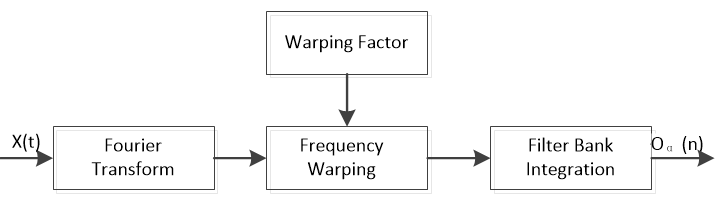
\includegraphics[width=6.0cm]{chapter4_figure/frequency_VTLN.png}}
 \centerline{(a)}\medskip
\end{minipage}
\hfill
\begin{minipage}[b]{0.48\linewidth}
  \centering
  \centerline{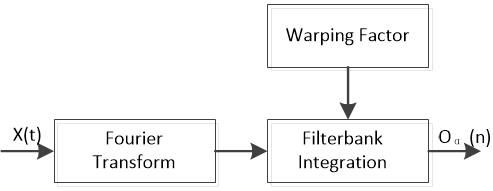
\includegraphics[width=4.0cm]{chapter4_figure/mel_VTLN.png}}
\centerline{(b)}\medskip
\end{minipage}
\caption{(a)Frequency warping VTLN (b)Mel scale VTLN}
\label{fig:res}
\end{figure}
÷�������ϵĹ�ʽ������ʾ��
\begin{equation}
O(n) = \sum_{\omega=l_{n}}^{\omega=h_{n}} T_{n}{\omega}X(\omega)   \qquad 0\le n\le N-1
\end{equation}
���У�$O(n)$�ǵ�n���˲����������N���˲����ĸ�����$T_{n}(\omega)$��n���˲�����$l_{n}$��$h_{n}$�ǵ�n���˲���$T_{n}(\omega)$�ĵ�ͨ���͸�ͨ����
���������÷��Ƶ������ʽ��ʾ��
\begin{equation}
v^{\alpha}_{l}=2595log(1+\alpha(f)/700)
\end{equation}
���У�$\alpha(f)$�ǹ��������� \\
���ۺ����������ԣ�linear�����ֶ�����(piecewise linear)��������(non-linear)��˫����(bilinear)����������$\alpha$���Ż�׼������������ʣ�maximum a posteriori probability��MAP��, ML, ��С������Minimum generation error��minimum MGE���ȡ�\\
ʹ��ML�Ż�׼�����ֶ����Ե��������ӡ�vocal Tract Length Normalization for Statistical Parametric Speech Synthesis��������ʽ��ʾ��
\begin{equation}
\hat{\alpha_{s}} =  arg \max \limits_{\alpha_{s}} p(x_{\alpha} | \Theta_{\alpha_{s}},\omega_{s})
\end{equation}
���У�$x_{\alpha_{s}}$��ʾ����˵����s���ۺ��������$\Theta$����ģ�ͣ�$\omega_{s}$��������˵����ת¼���ݣ� $\hat{\alpha_{s}}$��ʾ������ͬ˵������õ��������ӡ�\\
���Ͻ��ܵ��Ǵ�ͳ��VTLN��������Kaldi�У�ʹ�����Ա任����VTLN�����ֲ������ݵľ�ֵ��Э����䡾NOTES FOR AFFINE TRANSFORM-BASED VTLN��������ƽ��ڼ����Ϻܷ��㣬ֻҪ�����Ա任�������������������������Ա任�����־�ֵ��Э����仹��������Ҫԭ��:\\
(1)���Ա任���ܺܺõ��������۵��ס������������۵��ױ�ԭʼ���׷���Ҫ�ͣ�������ƥ���ƫ�ԭ���ķ�����ÿһά��һ��Э�������kaldi�У�ʹ����Э��������һ����\\
(2) �����Է�����log����ʽ�������Ӷ��ӽ�1��VTLN���ܺܲ��Ҫ����log����ʽ�ᣬ�����Աƽ���������Ҫ����log����ʽ����Ϊlog����ʽΪ0��
������������$x_{t}$,$1 \le t \le T$,$y_{t}^{(n)}$�����ۺ������������n���������࣬���־�ֵ��Э����䣬ͨ��ʹ$x_{t}^{+}$��$y_{t}^{(n)}$�����ܽӽ��������ת������$T^(n)$�������ܽ�һ�¼���ת������Ĺ�ʽ�� \\
x��ͳ��ֵ����ʽ��ʾ��
\begin{equation}
\bar{x} := \frac{1}{T} \sum_{t=1}^{T} x_{t}
\end{equation}
\begin{equation}
S := (\frac{1}{T} \sum_{t=1}^{T} x_{t}x_{t}^{T}) - \bar{x}\bar{x}^{T}
\end{equation}
Cholesky C����ʽ��ʾ��
\begin{equation}
S=CC^{T}
\end{equation}
P�Ĺ�ʽ������ʾ:
\begin{equation}
P_{0} := (\sum_{t=1}^{T} x_{t}y_{t}^{T}) - \bar{x} \sum_{t=1}^{T}y_{t}^{T}
\end{equation}
\begin{equation}
P=ULV^{T}
\end{equation}
���У�U��V�������ģ�L�ǶԽǾ���
\begin{equation}
N := VU^{T}
\end{equation}
\begin{equation}
M := CNC^{-1}
\end{equation}
\begin{equation}
v := \bar{x} - M\bar{x}
\end{equation}
\begin{equation}
T := [M;v]
\end{equation}
\subsection{����kaldi��VTLN}
VTLN��ͨ��compute-plp-feats,compute-fbank-feats,compute-mfcc-feats��һ��ѡ��"VTLN warp factor "ʵ�֡�
��kaldi�У�������һ��������\\
(1) ������������÷��Ƶ���ϣ�\\
(2) ���ۺ����������ķֶ����Ժ���;\\
(3) ����VtlnWarpFreq����ת�������������ۺ��Ƶ��;\\
(4) ���� MelScale�������ۺ��Ƶ�ʣ���Ƶ��ת��÷��Ƶ��
��ֹƵ������һ�¹�ϵ��\\
\begin{equation}
0 \le low\_freq \le vtln\_low   \le vtln\_high \le high\_freq  \le nyquist
\end{equation}
���У�$low\_freq$��$high\_freq$�������ĵ�Ƶ�͸�Ƶ��ֹƵ�ʣ�Ĭ��ֵ��Ϊ40��7800��$vtln\_low$��$vtln\_high$��vtln�ĵ�Ƶ�͸�Ƶ��ֹƵ��Ĭ��ֵ��Ϊ60,7200��nyquistĬ��ֵ��Ϊ8000��\\
���������ֳ����Σ������������$(high\_freq)$�����Ƶ��$(low\_freq)$Ϊ�ֽ�㡣$F(low\_freq)=low\_freq$ ,$F(high\_freq) =high\_freq$�����ۺ����������ġ�\\
��Ƶ����
\begin{equation}
scale\_low=(F_{l} - low\_freq) / (l - low\_freq)
\end{equation}
\begin{equation}
F(freq)=low\_freq + scale\_low * (freq - low\_freq)
\end{equation}
�м䣺\\
scale���� \\
\begin{equation}
W(freq)=scale * freq
\end{equation}
��Ƶ��:
\begin{equation}
scale\_high = (high\_freq - F_{h}) / (high\_freq - h)
\end{equation}
\begin{equation}
F(freq)=high\_freq + scale\_high * (freq - high\_freq)
\end{equation}
���У�scaleΪ�������ӵĵ���,l�����ۺ�����Ƶ��ֹƵ�ʣ�h�����ۺ�����Ƶ��ֹƵ�ʡ� \\
�����Ҫ��ʼ��VTLN�任��ʹ��gmm-init-vtln���\\
�÷�:\\
gmm-init-lvtln [options] $<lvtln-out>$ \\
����:\\
gmm-init-lvtln --dim=13 --num-classes=21 --default-class=10 1.lvtln \\

���ѵ��VTLN��ʹ��gmm-train-lvtln-special���\\
�÷�: \\
gmm-train-lvtln-special [options] class-index $<lvtln-in> <lvtln-out>  <feats-untransformed-rspecifier> <feats-transformed-rspecifier> [<posteriors-rspecifier>]$\\
����: \\
gmm-train-lvtln-special 5 5.lvtln 6.lvtln scp:train.scp scp:train\_warp095.scp ark:nosil.post \\
�������VTLNת�����󣬣�ʹ�þ���gmm-est-lvtln-trans���\\
�÷���\\
gmm-est-lvtln-trans [options] $<model-in> <lvtln-in> <feature-rspecifier> <gpost-rspecifier> <lvtln-trans-wspecifier> [<warp-wspecifier>]$
\section{PCA}
\subsection{PCA�Ļ���ԭ��}
���ɷַ�����principal components analysis, PCA����һ���޼ල�����Ա任�Ľ�ά�������ҵ���ά����֮������ڹ�ϵ��ͨ�����Ա任��ά�����͹۲�ռ��ά������ȡ����Ҫ����Ϣ��PCA��һ�����Ա任����ԭʼ���ݱ任��һ���µ�����ϵͳ�У���ԭʼ������������ͶӰ����󷽲���Ϊ��һ�����꣬����һ���ɷ֣��ڶ���ķ�����Ϊ�ڶ������꣬���ڶ����ɷ֣��Դ������¡����ɷָ�����ѡȡ�����趨�ۼƹ����ʣ����������ۼƷ�������ܷ���ı�ֵ����ˣ�PCA�����˵ͽ����ɷ֣����Ը߽����ɷ֣����������ݼ���ά���������˹����������ݼ�����A TUTORIAL ON PRINCIPAL COMPONENT ANALYSIS��\\
PCA��������ص�ԭʼ�������ת���ɷ�������ص��������������������Э�����ɶԽ���ԭ�������µ��������꣬���ݷֲ���P����������Ȼ��Զ�ά�������н�ά��
�������һ��PCA�任ԭ��:\\
(1) �����������$X_{1}��X_{2}��...��X_{p}$��������׼��$S_{1}��S_{2}��...��S_{p}$,����׼���任��
$C_{j}=a_{j1}x_{1}+a_{j2}x_{2}+...+a_{jp}x_{p}, j=1,2,...,p$\\
(2)��$C_{1}=a_{11}x_{1}+a_{12}x_{2}+...+a{1p}x_{p}$,��ʹ$Var(C_{1})$������$C_{1}$Ϊ��һ���ɷ֣�
(3)��$C_{2}=a_{21}x_{1}+a_{22}x_{2}+...+a{2p}x_{p}$,$(a_{21},a_{22},...,a_{2p})$��ֱ��$(a_{11},a_{12},...,a_{1p})$,��ʹ$Var(C_{2})$������$C_{2}$Ϊ��һ���ɷ֣�
(4) �Դ����ƣ��е��������ĵ���Ҫ�ɷ֣����p����\\
���ɷֵ����ʣ�\\
(1) ���ɷּ以����أ���������i��j��$C_{i}$��$C_{j}$�����ϵ��
\begin{equation}
Corr(C_{i},C_{j})=0
\end{equation}
(2) ���ϵ��$(a_{i1},a_{i2},...,a_{ip})$���ɵ�����Ϊ��λ������\\
(3) �����ɷֵķ���һ�εݼ��ģ���$Var(C_{1}) \ge Var(C_{2}) \ge ... \ge Var(C_{P}) $ \\
(4) �ܷ������������\\
$Var(C_{1})+Var(C_{2})+ ...+Var(C_{P})=Var(x_{1})+Var(x_{2})+...+Var(x_{p})$ \\

���ɷ���ԭ�������������,����Ϣ�����䡣\\
(5) ���ɷֺ�ԭ���������ϵ��$Corr(C_{i},x_{j})=a_{ij}$
(6) ��$X_{1}$��$X_{2}$��...��$X_{p}$����ؾ���ΪR��$(a_{i1},a_{i2},...,a_{ip})$������ؾ���R�ĵ�i����������������ֵ$l_{i}$���ǵ�i���ɷֵķ����$Var(C_{i})=l_{i}$,����$l_{i}$Ϊ��ؾ���R�ĵ�i������ֵ��\\
$l_{1} \ge l_{2} \ge... \ge l_{p}$
�����������ɷ�ȡ���ڱ����ɷֵ��ۼƷ����ڷ����ܺ�����ռ�ٷֱȣ�ʵ���У���Ϊ�趨һ���ٷֱȡ�\\
�����ܽ�һ�����ɷַ������ļ�����̣�\\
(1) �趨ԭʼ������mά�������$x=(X_{1},X_{2},...,X_{p})^{T}$,n������$xi=(x_{i1},x_{i2},...,x_{ip})^{T}, i=1,2,...,n$ ��$n\ge p$,��ԭʼ�������б�׼����
\begin{equation}
Z_{ij}=\frac {x_{ij}-\bar{x_{j}}}{s_{j}},i=1,2,...,p
\end{equation}
���У�$\bar{x_{j}}=\frac{\sum_{i=1}^{n} x_{ij}}{n},s^{2}_{j}=\frac{\sum_{i=1}^{n} (x_{ij}-\bar{x_{j}})^{2}}{n-1}$,�õ���׼������Z��\\
(2) �����׼������Z�����ϵ��
\begin{equation}
R=[r_{ij}]_{p} xp=\frac{Z^{T}Z}{n-1}
\end{equation}
����$r_{ij}=\frac{\Sigma z_{kj}*z_{kj}}{n-1},i,j=1,2,...,p$
(3)��������ؾ���R����������$|R-\lambda I_{p}|=0$,��p����������\\
��$\frac{\sum_{j=1}^{m}\lambda_{j}}{\sum_{j=1}^{p}\lambda_{j}} \ge 0.85$�������mֵ��\\
�ⷽ��$Rb=\lambda_{j}b$�õ���λ��������$b_{j}$
(4)����׼��������ת������õĵ�λ�������������ϣ�
 \begin{equation}
U_{ij}=z_{j}^{T}b_{j},j=1,2,...,m
\end{equation}
$U_{1}$��ʾ��һ�����ɷ֣�$U_{2}$��ʾ�ڶ������ɷ֣�...,$U_{p}$��ʾ��p�����ɷ֡�
\subsection{����Kaldi��PCA}
�������PCA�任��ʹ��est-pca���\\
�÷�:\\
est-pca [options] $(<feature-rspecifier>|<vector-rspecifier>) <pca-matrix-out>$ \\
���磺\\
$utils/shuffle_list.pl data/train/feats.scp | head -n 5000 | sort | est-pca --dim=50 scp:- some/dir/0.mat$ \\
\section{LDA}
\subsection{LDA�Ļ���ԭ��}
�����о�����(Linear Discriminant Analysis, LDA) ��һ�ַ��࣬��ά�����������任������LDA������һ�ּල��ѧϰ������������ǩ������ӳ�䵽��ά�ռ䣬ͶӰ�󵽵�ά�ռ�����ݰ���𻮷֣��任���������ԭ��������������ϡ�ͨ����������������ھ���ı�ֵ����������ֵ���֣�ʹ����󻯵ķ��ࡣ\\
�������ǽ���һ��LDA�����ļ�����̣�
�������ݼ�$\{{x_{i},y{i}}\}_{i=1}^{n}$������n���������������$x_{i} \in IR^{d}$��$y_{i} \in {1,2,...,k}$������i������������ǩ��d������ά����k�������������$X=[x_{1},x_{2},...,x_{n}]$���ֳ�k�࣬$X=[X_{1},X_{2},...,X_{K}]$,���У�$X_{j} \in IR^{d*n_{j}}$,$n_{j}$��j��$X_{j}$�ĸ���������$\sum_{j=1}^{k}n_{j}=n$��LDA�������Ա仯$F \in IR^{d*l}$���þ���dά��$x_{i}$ ӳ�䵽Lά��$x^{L}_{i}$����$x_{i} \in IR^{d} \to x^{L}_{i}=T^{T}x_{i} \in IR^{l} (l < d)$��\\
����ɢ������ֱ������ڣ���䣬��ɢ������ļ��㹫ʽ������ʾ��Least Squares Linear Discriminant Analysis�� ��LINEAR DISCRIMINANT ANALYSIS - A BRIEF TUTORIAL����\\
\begin{equation}
S_{\omega}=\frac{1}{n} \sum_{j=1}^{k} \sum_{x \in X_{j}} (x-c^{(j)})(x-c^{(j)})^{T}
\end{equation}
\begin{equation}
S_{b}=\frac{1}{n} \sum_{j=1}^{k} n_{j}(x-c^{(j)})(x-c^{(j)})^{T}
\end{equation}
\begin{equation}
S_{t}=\frac{1}{n} \sum_{j=1}^{k}(x-c^{(j)})(x-c^{(j)})^{T}
\end{equation}
���У�$c^{j}$�ǵ�j������ģ�c��ȫ�ֵ����ġ�����$S_{t}=S_{b}+S_{\omega}$��$trace(S_{\omega})$��ʾ���ھ��룬$trace(S_{b})$��ʾ�����롣�������Ա任T���õ���ά�ռ䣬����ɢ����������Ա任��������ʽ��ʾ��
\begin{equation}
S_{\omega}^{L}=T^{T}S_{\omega}T
\end{equation}
\begin{equation}
S_{b}^{L}=T^{T}S_{b}T
\end{equation}
\begin{equation}
S^{L}_{t}=T^{T}S_{t}T
\end{equation}
ͨ�����$trace(S^{L}_{b})$����С��$trace(S^{L}_{\omega})$���Ż����Ա任����T,����ͨ�����$trace(S^{L}_{b})$����С��$trace(S^{L}_{t})$���Ż����Ա任����T��\\
���Ա任�Ĺ�ʽ������ʾ��Least Squares Linear Discriminant Analysis����LINEAR DISCRIMINANT ANALYSIS - A BRIEF TUTORIAL����Two-Dimensional Linear Discriminant Analysis����
\begin{equation}
T^{LDA}=arg \max \limits_{T} \{trace(S_{b}^{L}(S^{L}_{t})^{-1})\}
\end{equation}
\begin{equation}
T^{LDA}=arg \min \limits_{T} \{trace((S_{b}^{L})^{-1})S_{\omega}^{L}\}
\end{equation}
���У�����ɢ�������Ƿ�����ģ�$G^{LDA}$��$S_{t}^{-1}S_{b}$�ķ�������ֵ��ɡ����ǣ�����ɢ������������ġ�$G^{LDA}$��$S_{t}^{+}S_{b}$�ķ�������ֵ��ɡ�$S^{+}_{t}$����$S_{t}$���棬��$S_{+}^{t}$����$S^{1}_{t}$��
�ϸ�С����ܵ�PCA��LDA���ǽ�ά��ȴ�ֲ�֮ͬ����\\
(1) PCA�����޼ලѧϰ����LDA�����мලѧϰ��\\
(2) PCA�Է���ĽǶȳ�������󷽲�Ϊ��һ���ɷ֡�Ȼ����LDA�ӷ���ĽǶȳ�������������������ھ�������ֵ���ҵ���÷����������\\
LDA��������һЩ�����ԣ� \\
(1) �����öԷǸ�˹�ֲ�������; \\
(2) ��������С������ά����ʹ���������ɢ�Ⱦ����������״�����õ���ͶӰ���������ŵ�; \\
(3) ���Ͻ��ܵ�LDA�Ծ�ֵΪ�ο�������Է���Ϊ�ο���ͶӰ����ķ��������ã� \\
(4) LDA�������ܳ��ֹ���������� \\
\subsection{����Kaldi��LDA}
����pdf-id����LDAͳ��ֵ��ʹ��acc-lda���\\
�÷���\\
acc-lda [options] $<transition-gmm/model> <features-rspecifier> <posteriors-rspecifier> <lda-acc-out> $ \\
���磺\\
ali-to-post $ark:1.ali ark:- | lda-acc 1.mdl "ark:splice-feats scp:train.scp|"  ark:- ldaacc.1$ \\
ʹ����ʽ�õ���LDAͳ��ֵ������LDA�任����ʹ��est-lda���\\
�÷���\\
est-lda [options] $<lda-matrix-out> <lda-acc-1> <lda-acc-2> ... $ \\

\section{DAE}
\subsection{DAE�Ļ���ԭ��}
����Ա���(Deep Autoencoder,DAE)��һ���޼ල���򴫲���ѧϰ�������ɱ������ͽ��������ɡ�SPEECH FEATURE DENOISING AND DEREVERBERATION VIA DEEP AUTOENCODERS FOR NOISY REVERBERANT SPEECH RECOGNITION����Stacked Denoising Autoencoders: Learning Useful Representations in a Deep Network with a Local Denoising Criterion�����趨������$\{x^{(1)},x^{(2)},...\}$������$x^{(i)} \in R^{n}$,DAEĿ��ֵ����DAE����ֵ����$y^{(i)}=x^{(i)}$��DAE��������һ��ѧϰ��ʹ���ֵ��������ֵ������������Ԫ�ĸ�����ȡ�DAE�ı���ӳ�亯������ʽ��ʾ:
\begin{equation}
f_{\theta} (x) = s(Wx+b)
\end{equation}
���У�$f_{\theta}$��nά������������������y��ӳ�亯��������$\theta=\{W,b\}$, W��$d*d$��Ȩ�ؾ���b��dά��ƫ��������\\
���ز�y�ع����������ӳ�������z��$z=g^{'}_{\theta}(y)$�����������DAE����,��ʽ����ʽ��ʾ��
\begin{equation}
g_{\theta}^{'}(y)=W^{'}y+b^{'}
\end{equation}
��ʽҲ����д��:
\begin{equation}
g_{\theta}^{'}(y)=s(W^{'}y+b^{'})
\end{equation}
���У�$\theta^{'}=\{W^{'},b^{'}\}$��z������׼ȷ�ع�x�����Ǽ���ֲ�����$p(X|Z=z)$��
�Ż��ع��������ع��������ʽ��ʾ:
\begin{equation}
L(x,z)=-logp(x|z)
\end{equation}
����ʵ��x,$X|z$����$N(z,\delta^{2}I)$,���Խ�L(x,z)��ʾ��:
\begin{equation}
L(x,z)=C(\delta^(2)) ||x-z||^{2}
\end{equation}
����$C(\delta^{2})$��ʾȡ����$\delta^{2}$���Ż�������\\

\subsection{����Kaldi��DAE}
���Ͻ��ܵĴ�ͳ��DAE������DAE�������룬�������������������ȣ�������������һ�����������൱��������ȡ��һ�����̣����������Ǵ��������ݣ���������Ǵ��������ݣ��Դ�������ΪѧϰĿ�꣬�ڴ�����Ҳ�Ǻܺ�ʵ�ֵġ�
����ԭʼDNNѵ���ű��������µĸĶ���
��1����Ŀ�꺯���ij���С��������(Mean Square Error,MSE)
��2��Ϊ�˱�֤����������MSEʱһ���ԣ�Ӧ��ȥ��softmax
��3��Ŀ�����������ʹ��feat-to-post���ת����kaldi�к�����ʵĸ�ʽ��
%%%%%%%%%%%%%%%%%%%%%%%%% referenc.tex %%%%%%%%%%%%%%%%%%%%%%%%%%%%%%
% sample references
% %
% Use this file as a template for your own input.
%
%%%%%%%%%%%%%%%%%%%%%%%% Springer-Verlag %%%%%%%%%%%%%%%%%%%%%%%%%%
%
% BibTeX users please use
% \bibliographystyle{}
% \bibliography{}
%
%\biblstarthook{In view of the parallel print and (chapter-wise) online publication of your book at \url{www.springerlink.com} it has been decided that -- as a genreral rule --  references should be sorted chapter-wise and placed at the end of the individual chapters. However, upon agreement with your contact at Springer you may list your references in a single seperate chapter at the end of your book. Deactivate the class option \texttt{sectrefs} and the \texttt{thebibliography} environment will be put out as a chapter of its own.\\\indent
%References may be \textit{cited} in the text either by number (preferred) or by author/year.\footnote{Make sure that all references from the list are cited in the text. Those not cited should be moved to a separate \textit{Further Reading} section or chapter.} The reference list should ideally be \textit{sorted} in alphabetical order -- even if reference numbers are used for the their citation in the text. If there are several works by the same author, the following order should be used:
%\begin{enumerate}
%\item all works by the author alone, ordered chronologically by year of publication
%\item all works by the author with a coauthor, ordered alphabetically by coauthor
%\item all works by the author with several coauthors, ordered chronologically by year of publication.
%\end{enumerate}
%The \textit{styling} of references\footnote{Always use the standard abbreviation of a journal's name according to the ISSN \textit{List of Title Word Abbreviations}, see \url{http://www.issn.org/en/node/344}} depends on the subject of your book:
%\begin{itemize}
%\item The \textit{two} recommended styles for references in books on \textit{mathematical, physical, statistical and computer sciences} are depicted in ~\cite{science-contrib, science-online, science-mono, science-journal, science-DOI} and ~\cite{phys-online, phys-mono, phys-journal, phys-DOI, phys-contrib}.
%\item Examples of the most commonly used reference style in books on \textit{Psychology, Social Sciences} are~\cite{psysoc-mono, psysoc-online,psysoc-journal, psysoc-contrib, psysoc-DOI}.
%\item Examples for references in books on \textit{Humanities, Linguistics, Philosophy} are~\cite{humlinphil-journal, humlinphil-contrib, humlinphil-mono, humlinphil-online, humlinphil-DOI}.
%\item Examples of the basic Springer style used in publications on a wide range of subjects such as \textit{Computer Science, Economics, Engineering, Geosciences, Life Sciences, Medicine, Biomedicine} are ~\cite{basic-contrib, basic-online, basic-journal, basic-DOI, basic-mono}.
%\end{itemize}
%}

\begin{thebibliography}{99.}%
% and use \bibitem to create references.
%
% Use the following syntax and markup for your references if
% the subject of your book is from the field
% "Mathematics, Physics, Statistics, Computer Science"
%
% Contribution
\bibitem{science-contrib} Broy, M.: Software engineering --- from auxiliary to key technologies. In: Broy, M., Dener, E. (eds.) Software Pioneers, pp. 10-13. Springer, Heidelberg (2002)
%
% Online Document
\bibitem{science-online} Dod, J.: Effective substances. In: The Dictionary of Substances and Their Effects. Royal Society of Chemistry (1999) Available via DIALOG. \\
\url{http://www.rsc.org/dose/title of subordinate document. Cited 15 Jan 1999}
%
% Monograph
\bibitem{science-mono} Geddes, K.O., Czapor, S.R., Labahn, G.: Algorithms for Computer Algebra. Kluwer, Boston (1992)
%
% Journal article
\bibitem{science-journal} Hamburger, C.: Quasimonotonicity, regularity and duality for nonlinear systems of partial differential equations. Ann. Mat. Pura. Appl. \textbf{169}, 321--354 (1995)
%
% Journal article by DOI
\bibitem{science-DOI} Slifka, M.K., Whitton, J.L.: Clinical implications of dysregulated cytokine production. J. Mol. Med. (2000) doi: 10.1007/s001090000086
%
\bigskip

% Use the following (APS) syntax and markup for your references if
% the subject of your book is from the field
% "Mathematics, Physics, Statistics, Computer Science"
%
% Online Document
\bibitem{phys-online} J. Dod, in \textit{The Dictionary of Substances and Their Effects}, Royal Society of Chemistry. (Available via DIALOG, 1999),
\url{http://www.rsc.org/dose/title of subordinate document. Cited 15 Jan 1999}
%
% Monograph
\bibitem{phys-mono} H. Ibach, H. L\"uth, \textit{Solid-State Physics}, 2nd edn. (Springer, New York, 1996), pp. 45-56
%
% Journal article
\bibitem{phys-journal} S. Preuss, A. Demchuk Jr., M. Stuke, Appl. Phys. A \textbf{61}
%
% Journal article by DOI
\bibitem{phys-DOI} M.K. Slifka, J.L. Whitton, J. Mol. Med., doi: 10.1007/s001090000086
%
% Contribution
\bibitem{phys-contrib} S.E. Smith, in \textit{Neuromuscular Junction}, ed. by E. Zaimis. Handbook of Experimental Pharmacology, vol 42 (Springer, Heidelberg, 1976), p. 593
%
\bigskip
%
% Use the following syntax and markup for your references if
% the subject of your book is from the field
% "Psychology, Social Sciences"
%
%
% Monograph
\bibitem{psysoc-mono} Calfee, R.~C., \& Valencia, R.~R. (1991). \textit{APA guide to preparing manuscripts for journal publication.} Washington, DC: American Psychological Association.
%
% Online Document
\bibitem{psysoc-online} Dod, J. (1999). Effective substances. In: The dictionary of substances and their effects. Royal Society of Chemistry. Available via DIALOG. \\
\url{http://www.rsc.org/dose/Effective substances.} Cited 15 Jan 1999.
%
% Journal article
\bibitem{psysoc-journal} Harris, M., Karper, E., Stacks, G., Hoffman, D., DeNiro, R., Cruz, P., et al. (2001). Writing labs and the Hollywood connection. \textit{J Film} Writing, 44(3), 213--245.
%
% Contribution
\bibitem{psysoc-contrib} O'Neil, J.~M., \& Egan, J. (1992). Men's and women's gender role journeys: Metaphor for healing, transition, and transformation. In B.~R. Wainrig (Ed.), \textit{Gender issues across the life cycle} (pp. 107--123). New York: Springer.
%
% Journal article by DOI
\bibitem{psysoc-DOI}Kreger, M., Brindis, C.D., Manuel, D.M., Sassoubre, L. (2007). Lessons learned in systems change initiatives: benchmarks and indicators. \textit{American Journal of Community Psychology}, doi: 10.1007/s10464-007-9108-14.
%
%
% Use the following syntax and markup for your references if
% the subject of your book is from the field
% "Humanities, Linguistics, Philosophy"
%
\bigskip
%
% Journal article
\bibitem{humlinphil-journal} Alber John, Daniel C. O'Connell, and Sabine Kowal. 2002. Personal perspective in TV interviews. \textit{Pragmatics} 12:257--271
%
% Contribution
\bibitem{humlinphil-contrib} Cameron, Deborah. 1997. Theoretical debates in feminist linguistics: Questions of sex and gender. In \textit{Gender and discourse}, ed. Ruth Wodak, 99--119. London: Sage Publications.
%
% Monograph
\bibitem{humlinphil-mono} Cameron, Deborah. 1985. \textit{Feminism and linguistic theory.} New York: St. Martin's Press.
%
% Online Document
\bibitem{humlinphil-online} Dod, Jake. 1999. Effective substances. In: The dictionary of substances and their effects. Royal Society of Chemistry. Available via DIALOG. \\
http://www.rsc.org/dose/title of subordinate document. Cited 15 Jan 1999
%
% Journal article by DOI
\bibitem{humlinphil-DOI} Suleiman, Camelia, Daniel C. O��Connell, and Sabine Kowal. 2002. `If you and I, if we, in this later day, lose that sacred fire...��': Perspective in political interviews. \textit{Journal of Psycholinguistic Research}. doi: 10.1023/A:1015592129296.
%
%
%
\bigskip
%
%
% Use the following syntax and markup for your references if
% the subject of your book is from the field
% "Computer Science, Economics, Engineering, Geosciences, Life Sciences"
%
%
% Contribution
\bibitem{basic-contrib} Brown B, Aaron M (2001) The politics of nature. In: Smith J (ed) The rise of modern genomics, 3rd edn. Wiley, New York
%
% Online Document
\bibitem{basic-online} Dod J (1999) Effective Substances. In: The dictionary of substances and their effects. Royal Society of Chemistry. Available via DIALOG. \\
\url{http://www.rsc.org/dose/title of subordinate document. Cited 15 Jan 1999}
%
% Journal article by DOI
\bibitem{basic-DOI} Slifka MK, Whitton JL (2000) Clinical implications of dysregulated cytokine production. J Mol Med, doi: 10.1007/s001090000086
%
% Journal article
\bibitem{basic-journal} Smith J, Jones M Jr, Houghton L et al (1999) Future of health insurance. N Engl J Med 965:325--329
%
% Monograph
\bibitem{basic-mono} South J, Blass B (2001) The future of modern genomics. Blackwell, London
%
\end{thebibliography}

\bibliographystyle{IEEEbib}
\bibliography{refs4}

\include{chapter5}
\include{chapter6}
\include{chapter7}
\include{chapter8}
\include{chapter9}
\include{chapter10}
\include{appendix}

\backmatter%%%%%%%%%%%%%%%%%%%%%%%%%%%%%%%%%%%%%%%%%%%%%%%%%%%%%%%
%\include{glossary}
%\include{solutions}
\printindex

%%%%%%%%%%%%%%%%%%%%%%%%%%%%%%%%%%%%%%%%%%%%%%%%%%%%%%%%%%%%%%%%%%%%%%

\end{document}





